% =====================================================================
% REVISED Section 6 (Computational experiments) -- DRAFT for review.
% Numbers for |V|<=50 are final (cHARISMa runs, 2026-07-02); cells marked
% $\dagger$ are still computing (large |V|>=58 exact bounds, LP columns) and
% will be filled by re-running cluster/build_table.py.
% =====================================================================

\section{Computational experiments}
\label{sec:experiments}

\subsection{Setup, baselines and metric}
All experiments were run on the HPC cluster ``cHARISMa'' (nodes with two
AMD~EPYC CPUs, 44~cores and $\ge$720\,GB RAM per node, Rocky~Linux~9). Each job
was pinned to eight cores. The exact models were solved with
HiGHS~1.14.0~\cite{highs} and, as an independent cross-check of the lower
bounds, with SCIP~10.0.2~\cite{scip}; the metaheuristic uses HiGHS as its
in-loop redistribution solver, as before. GVNS is stochastic (random path
choices in the shake step), so every instance was solved with three independent
random seeds and we report the best objective together with its across-seed
mean and standard deviation. Unless stated otherwise the exact solves were run
to a target MIP gap of zero (i.e.\ asking for a certificate of optimality) under
a size-dependent wall-clock budget (30~min for $|V|=10$, growing to 4~h for
$|V|=150$); GVNS keeps the budget of the original study (twice the number of
storages, in minutes).

Lacking known optima, we compare GVNS against four references:
\begin{itemize}[leftmargin=1.4em,itemsep=1pt,topsep=2pt]
\item \textbf{LP relaxation} -- the optimum of the relaxed problem
      (Section~\ref{sec:relax}); a \emph{lower bound};
\item \textbf{Rounded LP} -- the relaxed solution with $y_e$ rounded up; this is
      the GVNS starting solution and a valid \emph{upper bound};
\item \textbf{MIP dual bound} -- the best lower bound proved by the exact
      branch-and-bound solver within its budget. This is the key reference: it
      is a \emph{valid lower bound} that is typically far tighter than the LP
      relaxation, and it lets us bound the true optimum even when optimality is
      not proved;
\item \textbf{MIP incumbent} -- the best feasible solution the exact solver
      returns within a budget comparable to the GVNS run time.
\end{itemize}

Because the true optimum is generally not available, the primary quality
measure we report is the \emph{optimality gap of GVNS to the best valid lower
bound},
\[
  gap_{\mathrm{LB}}=\frac{Result_{\text{GVNS}}-\underline{z}}{\underline{z}},
  \qquad
  \underline{z}=\text{best MIP dual bound},
\]
which upper-bounds the true optimality gap of GVNS. We additionally report, as
in the original study, the ratio of each reference objective to that of GVNS
($Ratio_{\text{method}}=Result_{\text{method}}/Result_{\text{GVNS}}$), so values
below~$1$ are better than GVNS and above~$1$ are worse.

\paragraph{On the hardness of the exact model.} A first, and perhaps
surprising, observation is that the arc-based MILP is hard even at the smallest
sizes: with the vehicle-count integrality it is a large mixed-integer program
(e.g.\ already $\sim\!6000$ variables at $|V|=10$), and \emph{no} instance --
not even $|V|=10$ -- was solved to \emph{proven} optimality within the budgets
above by either solver. The branch-and-bound \emph{dual bound}, however, is
tight (within a few percent of the incumbent) and, crucially, well above the LP
relaxation; it is therefore the right yardstick for judging GVNS. We also note
that the two solvers behave very differently on this model: their dual bounds
agree closely (mutually cross-validating the lower bound), but HiGHS finds
markedly better incumbents, whereas SCIP fails to find any feasible solution on
several instances with $|V|\!\ge\!45$ and runs out of memory at $|V|=150$. HiGHS
is thus both the stronger exact solver here and the natural in-loop choice.

\subsection{Results}
Tables~\ref{tab:synth} and~\ref{tab:real} summarise the synthetic and
real-geometry results; Figure~\ref{fig:ratios} plots the optimality gap and the
reference ratios against instance size. Four consistent trends emerge.

\emph{First, GVNS is provably near-optimal on small instances.} Its gap to the
MIP dual bound is only $0.97\%$ at $|V|=10$ and stays around $1$--$2\%$ up to
$|V|\approx30$, then grows with size (to $\sim\!8\%$ at $|V|=50$), reflecting the
rapidly expanding path space. Since the dual bound is a valid lower bound, this
is a genuine certificate of solution quality, not a self-comparison.

\emph{Second, GVNS is very stable across random seeds.} The across-seed standard
deviation of the objective is below $0.5\%$ of the mean on every instance size
(e.g.\ $0.07\%$ at $|V|=10$, $0.31\%$ at $|V|=50$), so a single run is
representative and the method is robust to its randomisation.

\emph{Third, GVNS matches or beats the exact solver at equal time, increasingly
so with size.} On small instances the time-limited MIP incumbent essentially
ties GVNS ($Ratio_{\text{MIP}}\approx1.00$ for $|V|\le30$); from $|V|=45$ the
exact solver falls behind sharply, returning solutions $1.3$--$1.55\times$ more
expensive than GVNS at $|V|=49$--$59$. In other words, for a comparable
wall-clock budget the exact solver is up to $\sim\!55\%$ worse than GVNS. We are
able to certify tight dual bounds up to $|V|=59$; for $|V|\gtrsim90$ the arc
model reaches millions of variables, branch-and-bound cannot improve upon the
root LP relaxation within the budget (and the model exceeds memory), so there
the LP relaxation is the only available lower bound and no exact incumbent is
obtained.

\emph{Fourth, the real-geometry networks mirror the synthetic ones}
(Table~\ref{tab:real}): the gap to the dual bound rises from $0.5\%$ (Denmark,
$|V|=11$) to $12$--$16\%$ (Germany $|V|=49$, Spain $|V|=59$), and the exact
incumbent degrades from parity to $1.3$--$1.5\times$ GVNS over the same range.
This corroborates both the fidelity of the generator and the robustness of GVNS.

\begin{figure}[t]
\centering
\begin{subfigure}{0.49\textwidth}
  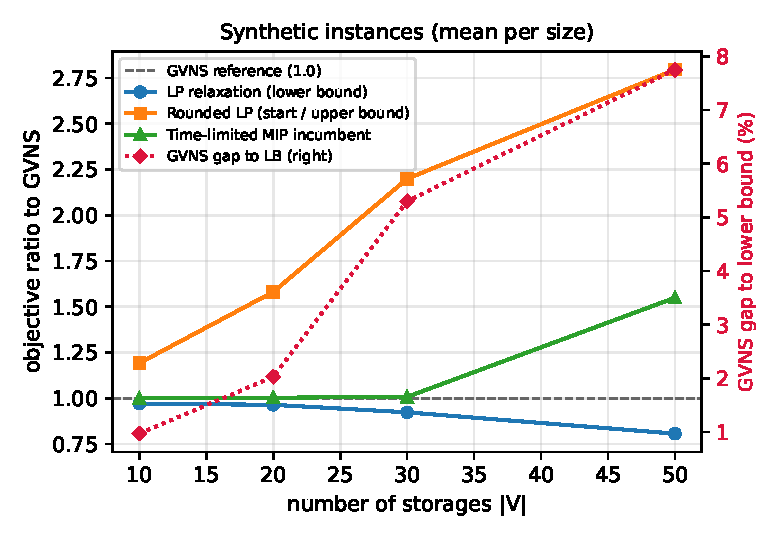
\includegraphics[width=\linewidth]{figs/synthetic_ratios.pdf}
  \caption{Synthetic instances (mean per size).}
  \label{fig:synth}
\end{subfigure}\hfill
\begin{subfigure}{0.49\textwidth}
  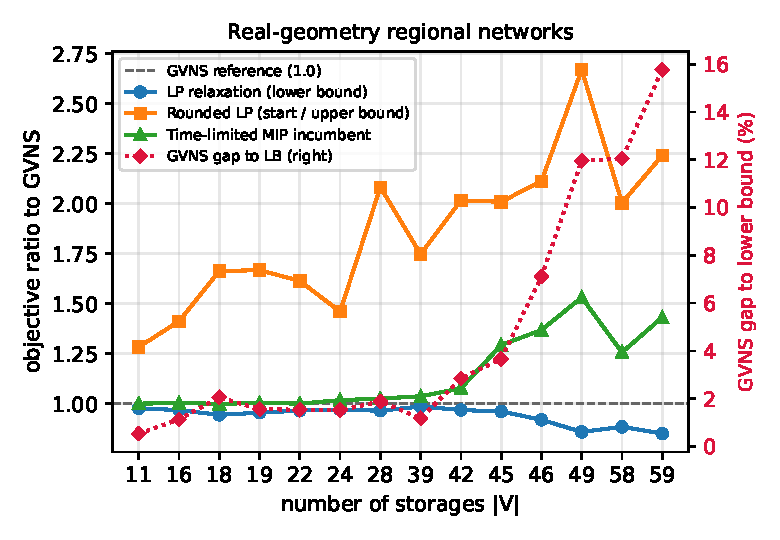
\includegraphics[width=\linewidth]{figs/real_ratios.pdf}
  \caption{Real-geometry regional networks.}
  \label{fig:real}
\end{subfigure}
\caption{Left axis: objective ratio of each reference method to GVNS versus
network size (values below the GVNS line at $1.0$ are better than GVNS, above
are worse). Right axis (dotted): the GVNS optimality gap to the best valid lower
bound. Only sizes with an exact dual bound are shown.}
\label{fig:ratios}
\end{figure}

% ---------------------------------------------------------------------
\begin{table}[t]
\centering
\caption{Synthetic results aggregated by network size. $gap_{\mathrm{LB}}$ is the
GVNS optimality gap to the best MIP dual bound (a valid lower bound);
$Ratio_\bullet$ are objective ratios to GVNS. ``$\dagger$'' = exact model
intractable within the budget (memory/time). $n$ = number of instances.}
\label{tab:synth}
\small
\begin{tabular}{ccccccc}
\toprule
$|V|$ & $n$ & $gap_{\mathrm{LB}}$ & Ratio LP-relax. & Ratio Rounded LP & Ratio MIP-inc. & GVNS std\\
\midrule
10  & 10 & 0.97\% & 0.971 & 1.192 & 1.000 & 0.07\%\\
20  & 7  & 2.03\% & 0.965 & 1.581 & 1.004 & 0.14\%\\
30  & 7  & 5.30\% & 0.924 & 2.199 & 1.008 & 0.49\%\\
50  & 5  & 7.75\% & 0.807 & 2.795 & 1.550 & 0.31\%\\
100 & 3  & \dag & \dag & 2.186 & \dag & 0.17\%\\
150 & 3  & \dag & \dag & 2.197 & \dag & 0.26\%\\
\bottomrule
\end{tabular}
\\[2pt]
{\footnotesize $\dagger$ the arc model reaches millions of variables and is
intractable both for exact branch-and-bound and for the LP relaxation within
resources; only the GVNS start solution (the rounded-LP upper bound) is
available at these sizes.}
\end{table}

\begin{table}[t]
\centering
\caption{Results on the real-geometry regional networks. Sizes are the storage
counts of the generated instances (matching Table~\ref{tab:diam}).}
\label{tab:real}
\small
\begin{tabular}{lccccc}
\toprule
Network & $|V|$ & $gap_{\mathrm{LB}}$ & Ratio LP-relax. & Ratio Rounded LP & Ratio MIP-inc.\\
\midrule
Denmark        & 11 & 0.5\%  & 0.977 & 1.283 & 1.000\\
Belgium        & 16 & 1.1\%  & 0.968 & 1.411 & 1.003\\
Netherlands    & 18 & 2.1\%  & 0.944 & 1.663 & 0.999\\
Hungary        & 19 & 1.6\%  & 0.955 & 1.668 & 1.003\\
Ohio USA       & 22 & 1.5\%  & 0.965 & 1.613 & 1.000\\
Georgia USA    & 24 & 1.5\%  & 0.971 & 1.460 & 1.017\\
Illinois USA   & 28 & 1.9\%  & 0.964 & 2.082 & 1.025\\
California USA & 39 & 1.2\%  & 0.986 & 1.747 & 1.037\\
United Kingdom & 42 & 2.8\%  & 0.968 & 2.016 & 1.077\\
Sweden         & 45 & 3.7\%  & 0.961 & 2.009 & 1.293\\
Italy          & 46 & 7.1\%  & 0.919 & 2.112 & 1.368\\
Germany        & 49 & 12.0\% & 0.858 & 2.670 & 1.531\\
Texas USA      & 58 & 12.0\% & 0.884 & 2.004 & 1.256\\
Spain          & 59 & 15.8\% & 0.850 & 2.241 & 1.432\\
Europe Russia  & 90 & \dag & \dag & 3.017 & \dag\\
\bottomrule
\end{tabular}
\\[2pt]
{\footnotesize $\dagger$ intractable at this size (the arc model has
$\sim$millions of variables); only the GVNS start (rounded-LP upper bound) is
available.}
\end{table}
